% !TEX program = xelatex

% Základní balíčky
\documentclass[10pt,a4paper]{article}
\usepackage[utf8]{inputenc}
\usepackage[czech]{babel}
\usepackage{graphicx}
\usepackage{wrapfig}
\usepackage{nonfloat}
\usepackage{cm-super}
\usepackage{amsmath}
\usepackage{hyperref}
\usepackage{gensymb}
\usepackage[top = 1cm, bottom = 1cm, left = 1cm, right = 1cm]{geometry}

% Bibtex
\usepackage{etoolbox}
\patchcmd{\thebibliography}{\section*{\refname}}{}{}{}

% Pro titulní stránku
\usepackage{titlesec}
\usepackage{setspace}
\usepackage{framed}
\usepackage{array}

% Vlastní balíčky
\usepackage{gnuplottex}
\usepackage{epstopdf}
\usepackage{csvsimple}
\usepackage{units}


\renewcommand{\U}[1]{\ensuremath{\,\mathrm{#1}}}
\newcommand{\°}{\degree}

\newcommand{\titjmeno}{Michal Grňo}
\newcommand{\titobor}{FOF}


\newcommand{\titcislo}{A21}
\newcommand{\titnazev}{Studium rentgenových spekter}
\newcommand{\titmereni}{11. 11. 2019}
\newcommand{\titodevzdani}{17. 11. 2019}


\begin{document}


\thispagestyle{empty}
\newgeometry{top = 2.5cm, bottom = 0cm, left = 2.5cm, right = 3cm}

{%T tomto je uzavřena celá titulka
%Tloušťka rámečku
\setlength{\fboxrule}{1.5pt}

\noindent
\framebox{
\begin{minipage}{\textwidth}
\setlength{\parindent}{17.62482 pt}
\phantom{d}

\begin{minipage}{0.6\textwidth}
{
\Large Kabinet výuky obecné fyziky, UK MFF\\
}
\vspace*{0.2cm}

{
\bfseries
\huge Fyzikální praktikum %ČÍSLO
}
\end{minipage}
\begin{minipage}{0.4\textwidth}
\begin{center}

\includegraphics[width=4.5cm]{ZFP.jpg}
\end{center}
\end{minipage}\\\\

%\vspace*{0.5cm}

{
\setstretch{1.5}
\Large
\noindent
Úloha č. \titcislo

\noindent
Název úlohy: \titnazev

\noindent
Jméno: \titjmeno
\hspace*{\fill}
Obor: \titobor

\noindent
Datum měření: \titmereni
\hspace*{\fill}
Datum odevzdání: \titodevzdani

\phantom{d}
}
\end{minipage}
}
%Konec horního rámečku

{
\phantom{d}

\Large
Připomínky opravujícího:\\
\vspace*{6.75cm}
}

\newcommand{\linka}{\noalign{\hrule height 1pt}}
\newcommand{\linkadva}{\noalign{\hrule height 1.5pt}}
\setlength\extrarowheight{9.5pt}
\Large
\noindent
\begin{tabular}{!{\vrule width 1.5pt} l !{\vrule width 1pt} c !{\vrule width 1pt} c !{\vrule width 1.5pt}}
\linkadva
   & Možný počet bodů & Udělený počet bodů \\\linkadva
  Práce při měření & 0-3 &  \\\linka
  Teoretická část & 0-2 &  \\\linka
  Výsledky a zpracování měření & 0-9 &  \\\linka
  Diskuse výsledků & 0-4 &  \\\linka
  Závěr & 0-1 &  \\\linka
  Použitá literatura & 0-1 &  \\\linkadva
  \hspace*{\fill} \textbf{Celkem} \hspace*{\fill}& max. 20 &  \\
\linkadva
\end{tabular}
\phantom{d}

Posuzoval: \hspace*{\fill}dne:~~~~~~~~~~~~~~~~~

}%Konec uzavření titulky
\newpage
\newgeometry{top = 2cm, bottom = 2cm, left = 2cm, right = 2cm}
\setcounter{page}{1}

\section{Pracovní úkoly}
\begin{enumerate}
    \item Proveďte energetickou kalibraci α-spektrometru a určete jeho rozlišení.
    \item Určete absolutní aktivitu kalibračního radioizotopu $^{241}$Am.
    \item Změřte závislost ionizačních ztrát α-částic na tlaku vzduchu $ΔT = ΔT(P)$.
    \item Určete specifické ionizační ztráty α-částic ve vzduchu při normálním tlaku $-dT/dx = f(T)$. Srovnejte tuto závislost se závislostí získanou pomocí empirické formule pro dolet α-částic ve vzduchu za normálních podmínek.
    \item Určete energie α-částic vyletujících ze vzorku obsahujícím izotop $^{239}$Pu a příměs izotopu $^{238}$Pu a porovnejte je s tabelovanými hodnotami. Stanovte relativní zastoupení izotopu $^{238}$Pu ve vzorku s přesností lepší než 10 \%, jsou-li $T_{1/2}({}^{238}Pu) = 87.71 \U{yr}$ a $T_{1/2}({}^{239}Pu) = 24.13 \cdot 10^3 \U{yr}$.
\end{enumerate}

\pagebreak

\section{Teoretická část}
V práci budeme měřit α-záření

\pagebreak
\section{Výsledky měření}
\phantom{.}\vspace{-\baselineskip}
\begin{wrapfigure}{r}{8cm}
    \centering
    \vspace{-\baselineskip}
    \begin{gnuplot}[terminal=epslatex,terminaloptions={color size 8cm, 5cm}]
        plot x
    \end{gnuplot}
    \vspace{-2\baselineskip}
    \caption{Způsob odečtu mezních úhlů, zde konkrétně u $^{29}$Cu při $20\U{kV}$.}

    \vspace{\baselineskip}

    \begin{gnuplot}[terminal=epslatex,terminaloptions={color size 8cm, 6.5cm}]
        plot x
    \end{gnuplot}
    \vspace{-2\baselineskip}
    \caption{Naměřené hodnoty Planckovy konstanty}
    \label{graf-planck}

    \vspace{2\baselineskip}

    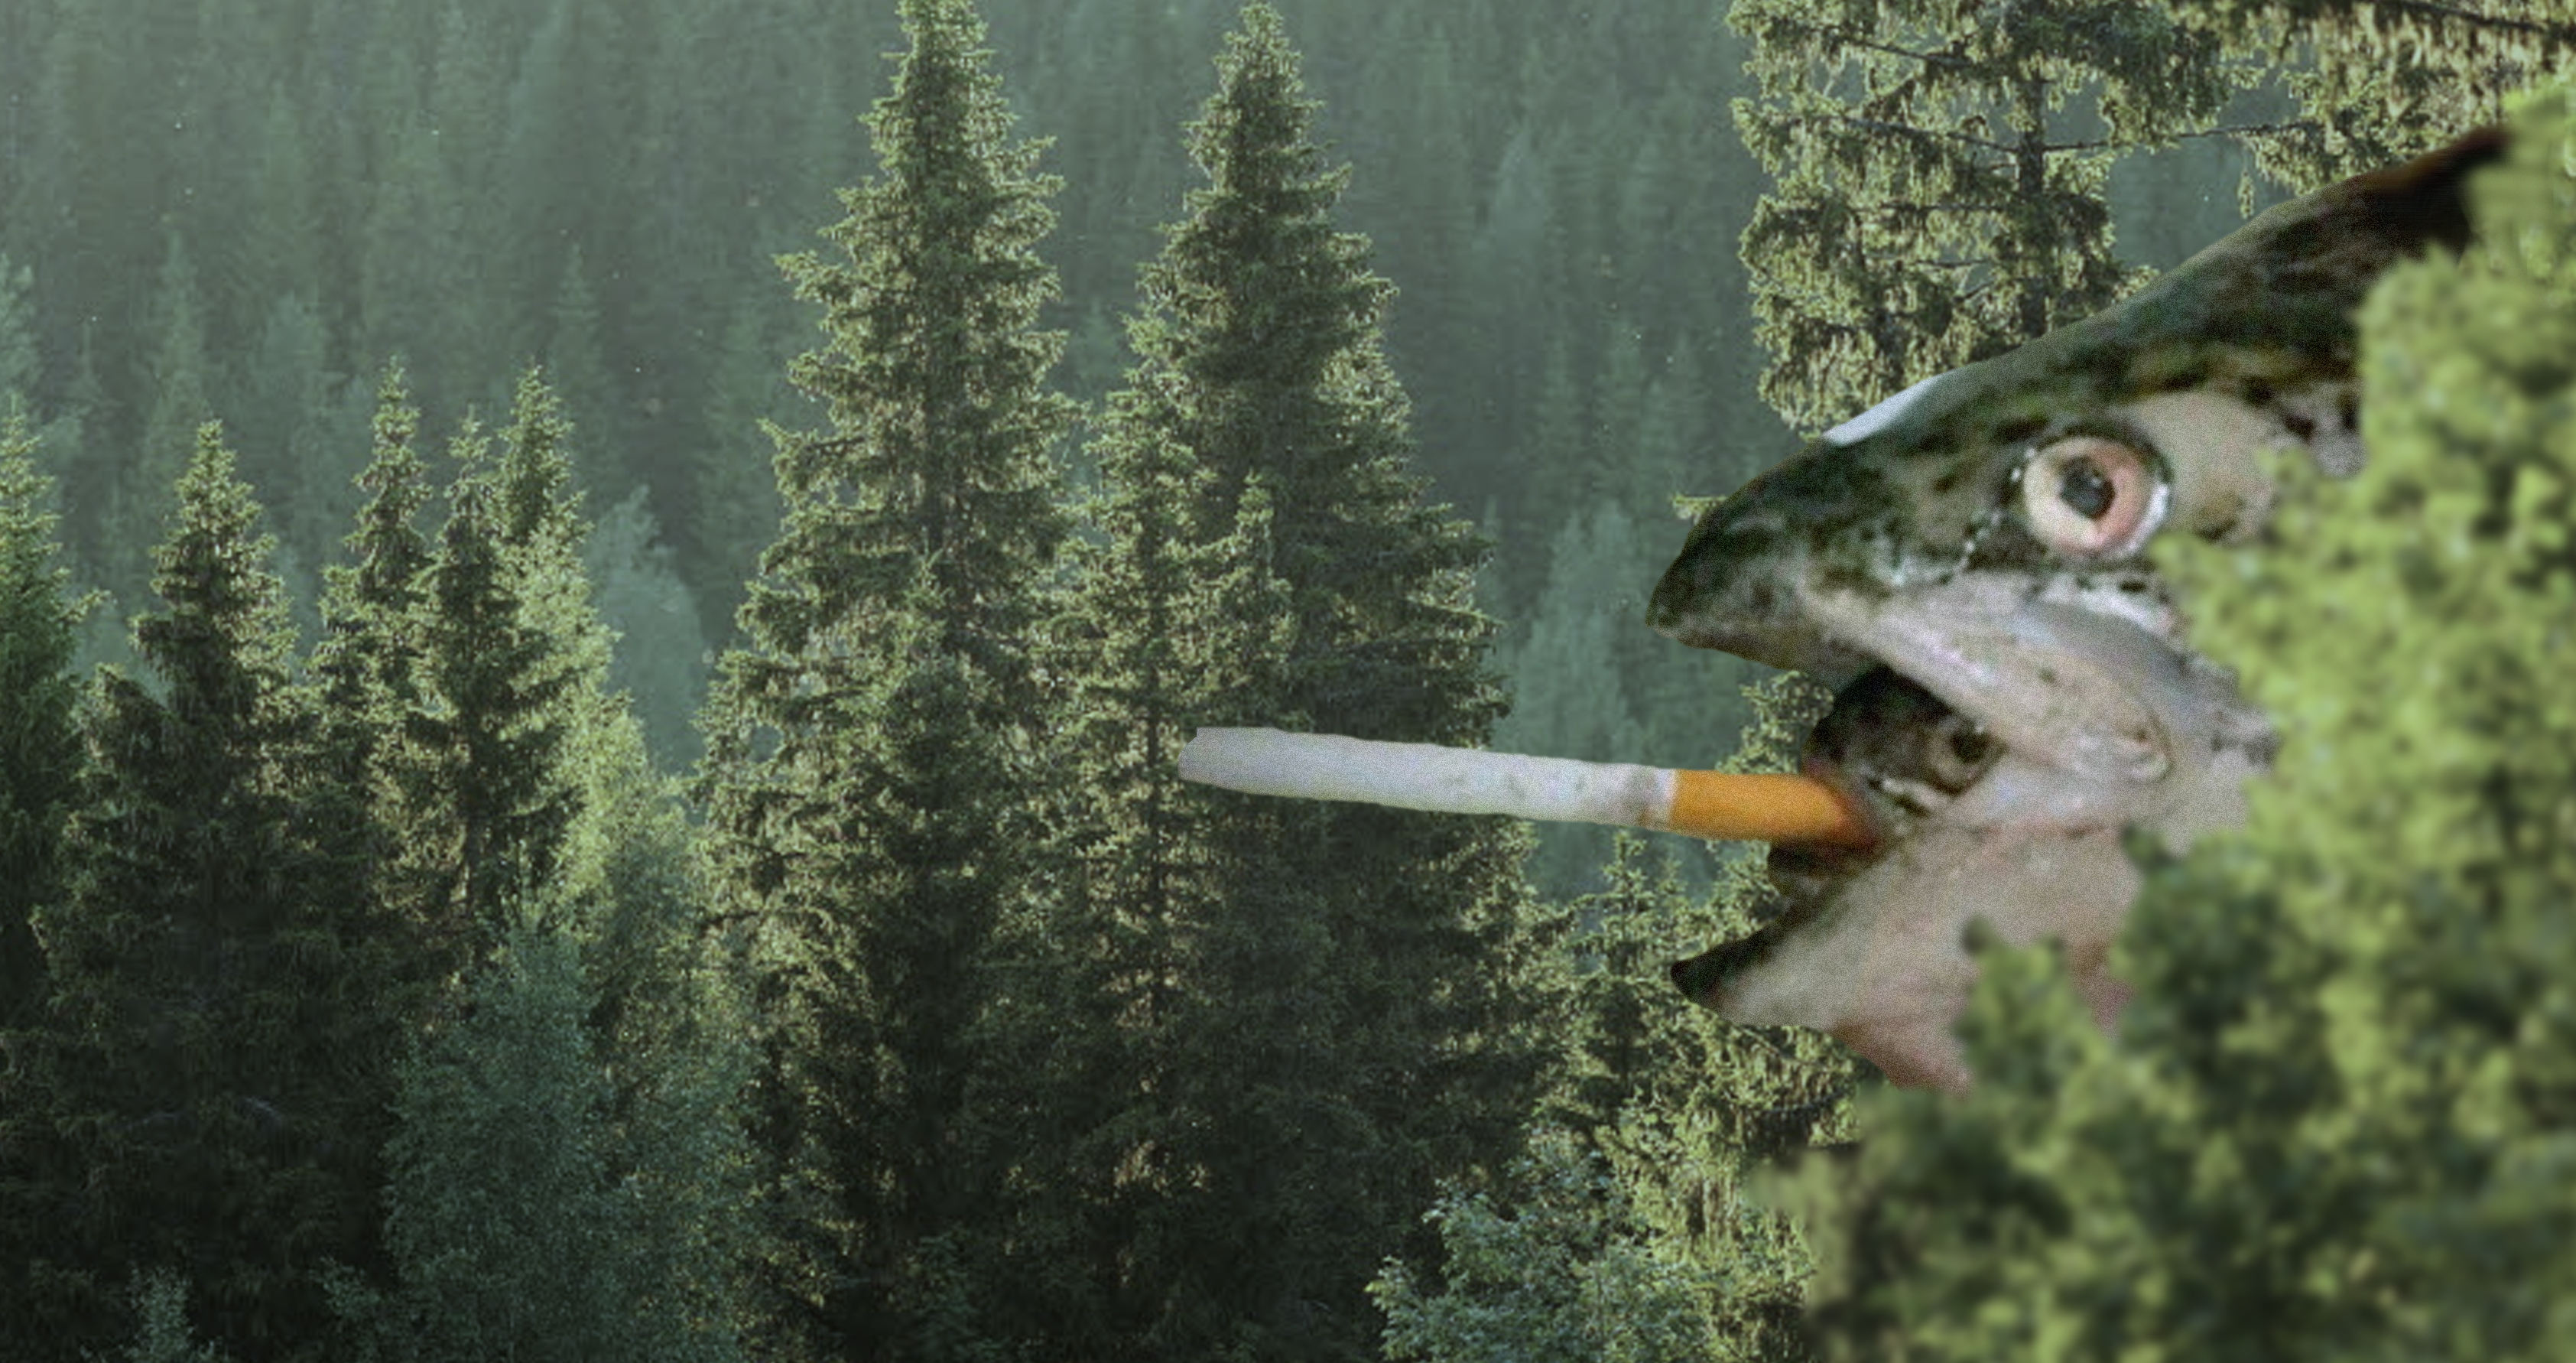
\includegraphics[width=7cm]{fish.jpeg}
    \vspace{-0.5\baselineskip}
    \caption{Pán lesa. Nepřeje si být rušen.}

    \vspace{2\baselineskip}

    \begin{gnuplot}[terminal=epslatex,terminaloptions={color size 8cm, 5cm}]
        plot x
    \end{gnuplot}
    \vspace{-2\baselineskip}
    \caption{Lineární závislost z \eqref{linearni-k-alpha} a \eqref{linearni-k-beta}}
    \vspace{-13cm}
    \label{graf-linearni}
\end{wrapfigure}
Nejprve jsme měřili brzdné záření na rentgence s měděnou anodou. Extrapolací z grafů jsme určili mezní úhly:
\begin{minipage}{\linewidth}
    \vspace{\baselineskip}
    \centering
    \begin{tabular}{ r|rl }
        \bfseries $U [\U{kV}]$ &
        \multicolumn{2}{c}{$\vartheta [\°]$}
        %\csvreader[ head to column names ]{data_brzdne.csv}{}
        %{
        %    \csviffirstrow{\\\hline}{\\}
        %    \valU & \valtheta & $\pm$ \valthetaerr
        %}
    \end{tabular}
    \vspace{\baselineskip}
    \tabcaption{Mezní úhly $\vartheta$}
    \label{mezni-uhly}
\end{minipage}

Autor připomíná, že $\vartheta$ značíme úhel ještě před korekcí na systematickou chybu. Úhel po korekci značíme ${\varphi = \vartheta + \vartheta_0}$.

Hodnoty Planckovy konstanty vypočtené podle \eqref{planck}, jejich průměř\footnote{Průměr je vážený převráceným čtvercem chyby.} a porovnání se skutečnou hodnotou je v grafu č. \ref{graf-planck}. Vidíme, že se skutečná hodnota signifikantně liší od té naměřené – to protože jsme zatím předpokládali, že systematická chyba $\vartheta_0 = 0$. Numericky nyní vyřešíme, pro jakou hodnotu $\vartheta_0$ se budou skutečná hodnota $h$ a vážený průměr rovnat. Získáme tím
\begin{equation}
    \vartheta_0 = 0.55 \°.
    \label{systematicka_chyba}
\end{equation}

Následně jsme měřili charakteristická spektra pro různé materiály anod. Pozorovali jsme maxima $n$-tého řádu na těchto úhlech:

\begin{minipage}{0.9\linewidth}
    \centering
    \vspace{\baselineskip}
    \begin{tabular}{ c|c|c|r|r }
        \multicolumn{1}{c|}{prvek} &
        \multicolumn{1}{c|}{$n$} &
        \multicolumn{1}{c|}{$U [\U{kV}]$} &
        \multicolumn{1}{c|}{$\theta(K_\alpha) [\°]$} &
        \multicolumn{1}{c}{$\theta(K_\beta) [\°]$}
        % \csvreader[ head to column names ]{data_charakt.csv}{}
        % {
        %     \csviffirstrow{\\\hline}{\\}
        %     $^{\valZ}$\prvek &
        %     \valn & \valU &
        %     \thetaalpha &
        %     \thetabeta
        % }
    \end{tabular}
    \vspace{\baselineskip}
    \tabcaption{Úhly $\vartheta$ maxim charakteristického záření}
    \label{charakt-uhly}
\end{minipage}

Použitím hodnot z tabulky \ref{charakt-uhly} a vypočtené systematické chyby z \eqref{systematicka_chyba} jsme sestavili graf \ref{graf-linearni}. Podle Moseleyova zákona má být vztah mezi $Z$ a $\sqrt{n/\sin\varphi}$ lineární.

Proložením z grafu jsme získali parametry fitu
% \csvreader[ head to column names ]{fity.csv.tmp}{}
% {
%     ${A(K_\alpha) = \valA}, \; {B(K_\alpha) = \valB}, \; {A(K_\beta) = \valC},$ ${B(K_\beta) = \valD}$
% }. Z toho jsme vypočetli hodnoty Rydbergových konstant:
\begin{align*}
    % \csvreader[ head to column names ]{rydberg.csv.tmp}{}
    % {
    %     K_\alpha: \; R_\omega &= \valalpha \cdot 10^{16} \U{s^{-1}}\\
    %     K_\beta: \; R_\omega &= \valbeta \cdot 10^{16} \U{s^{-1}}
    % }
\end{align*}

\pagebreak

\section{Diskuse}
Při měření se vyskytovala systematická chyba naměřeného úhlu. Ta byla korigována tak, aby $h$ vycházelo podle tabelovaných hodnot.

V grafu $I(\vartheta)$ závislosti intenzity na úhlu jsme pro velmi malé úhly pozorovali zesílení šumu – to bylo způsobeno faktem, že nemáme dokonale směrový zdroj ani detektor, detekovali jsme tedy záření, které nebylo difraktováno, ale doletělo do detektoru přímo. Pro vyšší úhly, tedy tam, kde jsme měřili hodnoty potřebné pro experiment, už tento jev neměl vliv.

Z grafu na obrázku č. \ref{graf-linearni} je vidět, že směrnice přechodů $K_\alpha$ a $K_\beta$ jsou jiné. To je pravděpodobně dáno tím, že Rydbergův vztah je pro všechny atomy, které nejsou vodík, pouze přibližný. I vypočtené hodnoty Rydbergovy konstatnty jsou kvůli tomu velmi odlišné pro $K_\alpha$ a $K_\beta$.


\section{Závěr}
Podařilo se vypočítat hodnotu Planckovy konstanty, jejím porovnáním se skutečnou hodnotou se podařilo určit systematickou chybu úhlu $\vartheta_0 = 0.55 \°$.

Podařilo se ověřit platnost Moseleyova zákona. Rydbergovy konstanty, které vyšly byly:
\begin{align*}
    % \csvreader[ head to column names ]{rydberg.csv.tmp}{}
    % {
    %     K_\alpha: \; R_\omega &= \valalpha \cdot 10^{16} \U{s^{-1}}\\
    %     K_\beta: \; R_\omega &= \valbeta \cdot 10^{16} \U{s^{-1}}
    % }
\end{align*}
Jejich průměr je tedy $R_\omega = (2.1 \pm 0.5) \cdot 10^{16} \U{s^{-1}}$. Skutečná hodnota Rydbergovy konstanty je:
\begin{equation*}
    R_\omega = 2.0606 \cdot 10^{16} \U{s^{-1}}
\end{equation*}




\section{Literatura}
[1] Studijní texty k laboratorní úloze: Studium rentgenových spekter; Kolektiv autorů ZFP KVOF MFF UK, online zdroj, [cit. 20.11.2019], dostupné na stránkách fyzikálního praktika IV

\end{document}